\documentclass{article}
\usepackage[utf8]{inputenc}
\usepackage[english]{babel}
\usepackage{amsmath}
\usepackage{amsfonts}
\usepackage{amssymb}
\usepackage{graphicx}
\usepackage{wrapfig}

\author{Arian Stolwijk}
\begin{document}

\section{Problem Description}

\begin{wrapfigure}{r}{0.4\textwidth}
  \vspace{-30pt}
  \begin{center}
    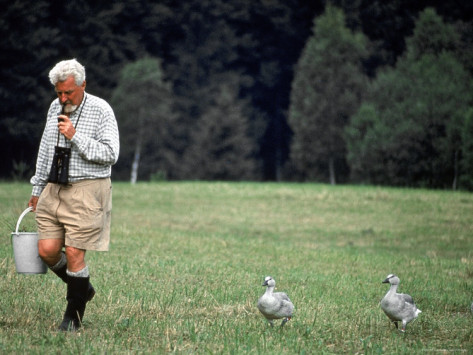
\includegraphics[width=0.38\textwidth]{geese.jpg}
    \vspace{-20pt}
  \end{center}
  \caption{Geese following a person}
\label{fig:geese}
\end{wrapfigure}

When a goose comes out of their eggs, it assumes its mother to be the first
thing it sees. Usually this is true and then it follows the mother for ever.
However if this is a human, it will simply follow the human too, as seen in
figure~\ref{fig:geese}.

Using a smartphone and a simple robot we can simulate the same effect. The
smartphone as mother and the robot as baby goose. The objective of the robot is
to follow the smartphone.

We will build a smartphone application that controls an extremely Arduino
robot. This robot can move forward, backwards, left or right. The smartphone
sends commands over Bluetooth to the robot to which direction the robot should
go. The robot blindly follows the commands, the smartphone is the smart
component in this setup. For the smarthpone to be smart it should know where
the robot is: the localization of the robot.

\section{Sensors to be used}

Localization of the robot is not a trivial thing to do, we need to combine
multiple sensors of the smartphone to achieve an accurate estimate of the
location of the robot. However besides the location the phone also needs to
know the orientation of the robot, to know whether it should send forward,
backwards, left or right commands to the robot.

First we will use the camera to get an initial belief. Using object tracking
we can get a \emph{Transformation Matrix} of the robot relative to the phone.

However if you rotate your phone and the robot is not in the camara viewport
anymore, the position should be saved. Using the orientation from the phone,
derived from the accelerometer and gyroscope, we can compensate for that.

You cannot always point your camera to the robot, which is impractical in many
cases. Instead you just want to put your phone back into your pocket and the
robot should still follow you. If you start walking or running in a direction,
the robot should follow. The accelerometer will be used to detect the current
activity.

Bluetooth will be used for communication, but also the Received Signal Strength
Indication (RSSI) can be used. If the strength increases or decreases indicates
if the distance to the robot is increasing or decreasing.

\section{Theoretical methods to be used}

We need image processing to detect the location and rotation of the robot with
the camera. Existing libraries exists, such as OpenCV, that can detect features
in an image. With three detected points the transformation can be constructed
using equation~(\ref{eq:transformation}).

\begin{equation}
A_{i} \times T_{i} = B_{i}
\label{eq:transformation}
\end{equation}

The $A_{i}$ matrix a reference point, while $B_{i}$ is the measured point. By
solving the equation the transformation can be calculated.

Using a particle filter we can have a probabilistic model where the robot is
relative to the smartphone.

Combining the Bluetooth RSSI and acceleration data we can change the particle
filter density function. For example if the RSSI decreases it means the user is
moving away from the robot so it is probably behind the user, and vice versa.

If the phone detects that the user is walking in a direction, it can also
adjust the density function, depending on the direction. To know whether the
user is walking, we can use the accelerometer. From the accelerometer a feature
vector can be extracted, with features such as zero-crossing frequency: how
many times the values pass zero, and the amplitude: what's the average
amplitude of the data. Having a feature vector the kNN classification method
can be used using calibration data to classify standing, walking or running.

\section{Initial Results}

We have started working on an Android Application. We defined the requirements
and specifications how the app can and should work. Further we started
implementing small initial parts of the app, such as reading sensors from the
accelerometer, camera and Bluetooth.

\end{document}

